\documentclass{extbook}[14pt]
\usepackage{multicol, enumerate, enumitem, hyperref, color, soul, setspace, parskip, fancyhdr, amssymb, amsthm, amsmath, latexsym, units, mathtools}
\everymath{\displaystyle}
\usepackage[headsep=0.5cm,headheight=0cm, left=1 in,right= 1 in,top= 1 in,bottom= 1 in]{geometry}
\usepackage{dashrule}  % Package to use the command below to create lines between items
\newcommand{\litem}[1]{\item #1

\rule{\textwidth}{0.4pt}}
\pagestyle{fancy}
\lhead{}
\chead{Answer Key for Progress Quiz 9 Version C}
\rhead{}
\lfoot{9541-5764}
\cfoot{}
\rfoot{Summer C 2021}
\begin{document}
\textbf{This key should allow you to understand why you choose the option you did (beyond just getting a question right or wrong). \href{https://xronos.clas.ufl.edu/mac1105spring2020/courseDescriptionAndMisc/Exams/LearningFromResults}{More instructions on how to use this key can be found here}.}

\textbf{If you have a suggestion to make the keys better, \href{https://forms.gle/CZkbZmPbC9XALEE88}{please fill out the short survey here}.}

\textit{Note: This key is auto-generated and may contain issues and/or errors. The keys are reviewed after each exam to ensure grading is done accurately. If there are issues (like duplicate options), they are noted in the offline gradebook. The keys are a work-in-progress to give students as many resources to improve as possible.}

\rule{\textwidth}{0.4pt}

\begin{enumerate}\litem{
Construct the lowest-degree polynomial given the zeros below. Then, choose the intervals that contain the coefficients of the polynomial in the form $ax^3+bx^2+cx+d$.
\[ \frac{4}{3}, \frac{2}{3}, \text{ and } \frac{3}{5} \]The solution is \( 45x^{3} -117 x^{2} +94 x -24 \), which is option A.\begin{enumerate}[label=\Alph*.]
\item \( a \in [43, 49], b \in [-121, -109], c \in [94, 102], \text{ and } d \in [-30, -23] \)

* $45x^{3} -117 x^{2} +94 x -24$, which is the correct option.
\item \( a \in [43, 49], b \in [115, 126], c \in [94, 102], \text{ and } d \in [24, 25] \)

$45x^{3} +117 x^{2} +94 x + 24$, which corresponds to multiplying out $(3x + 4)(3x + 2)(5x + 3)$.
\item \( a \in [43, 49], b \in [2, 5], c \in [-61, -52], \text{ and } d \in [24, 25] \)

$45x^{3} +3 x^{2} -58 x + 24$, which corresponds to multiplying out $(3x + 4)(3x -2)(5x -3)$.
\item \( a \in [43, 49], b \in [63, 65], c \in [-21, -6], \text{ and } d \in [-30, -23] \)

$45x^{3} +63 x^{2} -14 x -24$, which corresponds to multiplying out $(3x + 4)(3x + 2)(5x -3)$.
\item \( a \in [43, 49], b \in [-121, -109], c \in [94, 102], \text{ and } d \in [24, 25] \)

$45x^{3} -117 x^{2} +94 x + 24$, which corresponds to multiplying everything correctly except the constant term.
\end{enumerate}

\textbf{General Comment:} To construct the lowest-degree polynomial, you want to multiply out $(3x -4)(3x -2)(5x -3)$
}
\litem{
Describe the end behavior of the polynomial below.
\[ f(x) = 8(x - 9)^{5}(x + 9)^{10}(x - 3)^{3}(x + 3)^{5} \]The solution is the graph below, which is option D.
    \begin{center}
        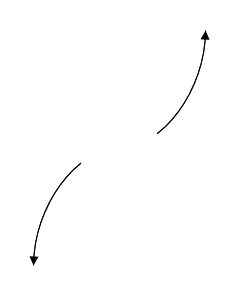
\includegraphics[width=0.3\textwidth]{../Figures/polyEndBehaviorCopyDC.png}
    \end{center}\begin{enumerate}[label=\Alph*.]
\begin{multicols}{2}
\item 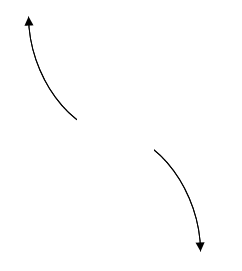
\includegraphics[width = 0.3\textwidth]{../Figures/polyEndBehaviorCopyAC.png}
\item 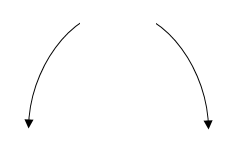
\includegraphics[width = 0.3\textwidth]{../Figures/polyEndBehaviorCopyBC.png}
\item 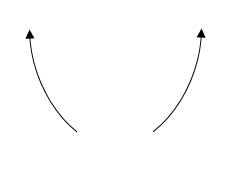
\includegraphics[width = 0.3\textwidth]{../Figures/polyEndBehaviorCopyCC.png}
\item 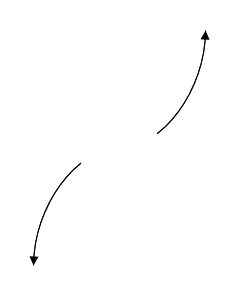
\includegraphics[width = 0.3\textwidth]{../Figures/polyEndBehaviorCopyDC.png}
\end{multicols}\item None of the above.\end{enumerate}
\textbf{General Comment:} Remember that end behavior is determined by the leading coefficient AND whether the \textbf{sum} of the multiplicities is positive or negative.
}
\litem{
Construct the lowest-degree polynomial given the zeros below. Then, choose the intervals that contain the coefficients of the polynomial in the form $x^3+bx^2+cx+d$.
\[ 2 + 4 i \text{ and } 1 \]The solution is \( x^{3} -5 x^{2} +24 x -20 \), which is option C.\begin{enumerate}[label=\Alph*.]
\item \( b \in [4.8, 7.3], c \in [22.72, 24.73], \text{ and } d \in [18.8, 23.2] \)

$x^{3} +5 x^{2} +24 x + 20$, which corresponds to multiplying out $(x-(2 + 4 i))(x-(2 - 4 i))(x + 1)$.
\item \( b \in [-0.5, 1.6], c \in [-4.03, -2.68], \text{ and } d \in [0.5, 2.3] \)

$x^{3} + x^{2} -3 x + 2$, which corresponds to multiplying out $(x -2)(x -1)$.
\item \( b \in [-8.6, -2.1], c \in [22.72, 24.73], \text{ and } d \in [-21.3, -19.8] \)

* $x^{3} -5 x^{2} +24 x -20$, which is the correct option.
\item \( b \in [-0.5, 1.6], c \in [-5.22, -3.99], \text{ and } d \in [2.7, 7] \)

$x^{3} + x^{2} -5 x + 4$, which corresponds to multiplying out $(x -4)(x -1)$.
\item \( \text{None of the above.} \)

This corresponds to making an unanticipated error or not understanding how to use nonreal complex numbers to create the lowest-degree polynomial. If you chose this and are not sure what you did wrong, please contact the coordinator for help.
\end{enumerate}

\textbf{General Comment:} Remember that the conjugate of $a+bi$ is $a-bi$. Since these zeros always come in pairs, we need to multiply out $(x-(2 + 4 i))(x-(2 - 4 i))(x-(1))$.
}
\litem{
Which of the following equations \textit{could} be of the graph presented below?

\begin{center}
    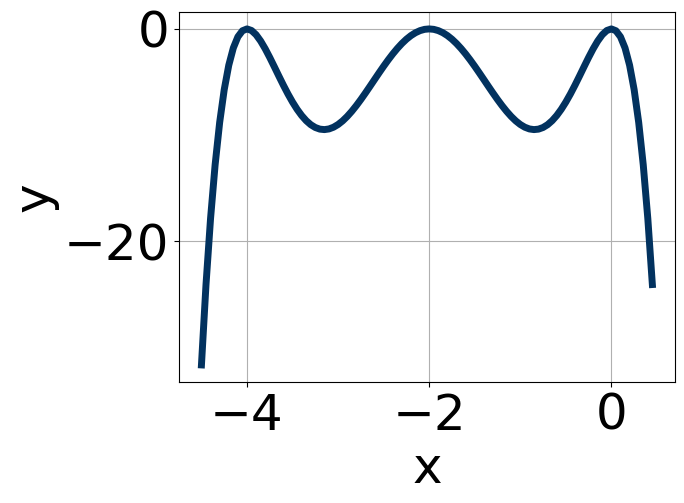
\includegraphics[width=0.5\textwidth]{../Figures/polyGraphToFunctionCopyC.png}
\end{center}


The solution is \( -3x^{4} (x + 2)^{8} (x + 4)^{8} \), which is option D.\begin{enumerate}[label=\Alph*.]
\item \( 18x^{5} (x + 2)^{8} (x + 4)^{4} \)

The factor $x$ should have an even power and the leading coefficient should be the opposite sign.
\item \( 9x^{10} (x + 2)^{8} (x + 4)^{6} \)

This corresponds to the leading coefficient being the opposite value than it should be.
\item \( -6x^{5} (x + 2)^{8} (x + 4)^{6} \)

The factor $x$ should have an even power.
\item \( -3x^{4} (x + 2)^{8} (x + 4)^{8} \)

* This is the correct option.
\item \( -14x^{5} (x + 2)^{6} (x + 4)^{5} \)

The factors $(x + 4)$ and $x$ should both have even powers.
\end{enumerate}

\textbf{General Comment:} General Comments: Draw the x-axis to determine which zeros are touching (and so have even multiplicity) or cross (and have odd multiplicity).
}
\litem{
Describe the zero behavior of the zero $x = 9$ of the polynomial below.
\[ f(x) = 9(x - 3)^{11}(x + 3)^{8}(x - 9)^{10}(x + 9)^{9} \]The solution is the graph below, which is option C.
    \begin{center}
        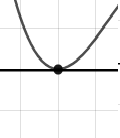
\includegraphics[width=0.3\textwidth]{../Figures/polyZeroBehaviorCopyCC.png}
    \end{center}\begin{enumerate}[label=\Alph*.]
\begin{multicols}{2}
\item 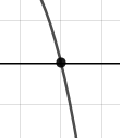
\includegraphics[width = 0.3\textwidth]{../Figures/polyZeroBehaviorCopyAC.png}
\item 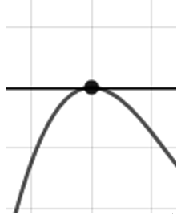
\includegraphics[width = 0.3\textwidth]{../Figures/polyZeroBehaviorCopyBC.png}
\item 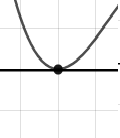
\includegraphics[width = 0.3\textwidth]{../Figures/polyZeroBehaviorCopyCC.png}
\item 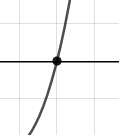
\includegraphics[width = 0.3\textwidth]{../Figures/polyZeroBehaviorCopyDC.png}
\end{multicols}\item None of the above.\end{enumerate}
\textbf{General Comment:} You will need to sketch the entire graph, then zoom in on the zero the question asks about.
}
\litem{
Describe the zero behavior of the zero $x = 4$ of the polynomial below.
\[ f(x) = 5(x + 6)^{5}(x - 6)^{4}(x + 4)^{9}(x - 4)^{6} \]The solution is the graph below, which is option C.
    \begin{center}
        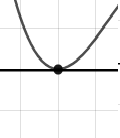
\includegraphics[width=0.3\textwidth]{../Figures/polyZeroBehaviorCC.png}
    \end{center}\begin{enumerate}[label=\Alph*.]
\begin{multicols}{2}
\item 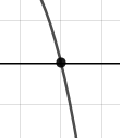
\includegraphics[width = 0.3\textwidth]{../Figures/polyZeroBehaviorAC.png}
\item 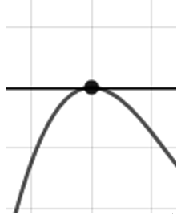
\includegraphics[width = 0.3\textwidth]{../Figures/polyZeroBehaviorBC.png}
\item 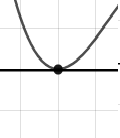
\includegraphics[width = 0.3\textwidth]{../Figures/polyZeroBehaviorCC.png}
\item 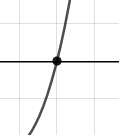
\includegraphics[width = 0.3\textwidth]{../Figures/polyZeroBehaviorDC.png}
\end{multicols}\item None of the above.\end{enumerate}
\textbf{General Comment:} You will need to sketch the entire graph, then zoom in on the zero the question asks about.
}
\litem{
Describe the end behavior of the polynomial below.
\[ f(x) = 2(x + 4)^{3}(x - 4)^{8}(x - 5)^{5}(x + 5)^{6} \]The solution is the graph below, which is option C.
    \begin{center}
        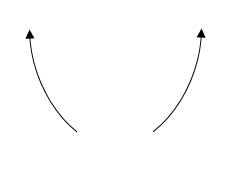
\includegraphics[width=0.3\textwidth]{../Figures/polyEndBehaviorCC.png}
    \end{center}\begin{enumerate}[label=\Alph*.]
\begin{multicols}{2}
\item 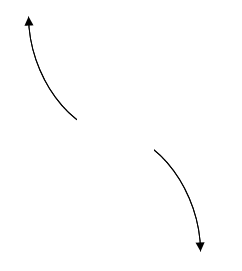
\includegraphics[width = 0.3\textwidth]{../Figures/polyEndBehaviorAC.png}
\item 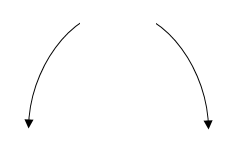
\includegraphics[width = 0.3\textwidth]{../Figures/polyEndBehaviorBC.png}
\item 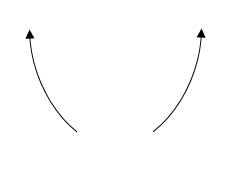
\includegraphics[width = 0.3\textwidth]{../Figures/polyEndBehaviorCC.png}
\item 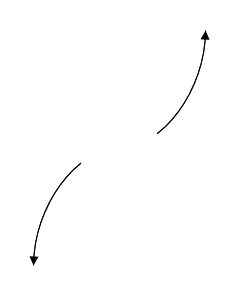
\includegraphics[width = 0.3\textwidth]{../Figures/polyEndBehaviorDC.png}
\end{multicols}\item None of the above.\end{enumerate}
\textbf{General Comment:} Remember that end behavior is determined by the leading coefficient AND whether the \textbf{sum} of the multiplicities is positive or negative.
}
\litem{
Construct the lowest-degree polynomial given the zeros below. Then, choose the intervals that contain the coefficients of the polynomial in the form $x^3+bx^2+cx+d$.
\[ -4 - 3 i \text{ and } 1 \]The solution is \( x^{3} +7 x^{2} +17 x -25 \), which is option C.\begin{enumerate}[label=\Alph*.]
\item \( b \in [-2.3, 1.9], c \in [1.81, 2.56], \text{ and } d \in [-3.42, -2.96] \)

$x^{3} + x^{2} +2 x -3$, which corresponds to multiplying out $(x + 3)(x -1)$.
\item \( b \in [-8.3, -5.2], c \in [15.94, 17.54], \text{ and } d \in [24.44, 26.01] \)

$x^{3} -7 x^{2} +17 x + 25$, which corresponds to multiplying out $(x-(-4 - 3 i))(x-(-4 + 3 i))(x + 1)$.
\item \( b \in [4.9, 8.8], c \in [15.94, 17.54], \text{ and } d \in [-26.86, -23.36] \)

* $x^{3} +7 x^{2} +17 x -25$, which is the correct option.
\item \( b \in [-2.3, 1.9], c \in [2.49, 3.29], \text{ and } d \in [-4.03, -3.82] \)

$x^{3} + x^{2} +3 x -4$, which corresponds to multiplying out $(x + 4)(x -1)$.
\item \( \text{None of the above.} \)

This corresponds to making an unanticipated error or not understanding how to use nonreal complex numbers to create the lowest-degree polynomial. If you chose this and are not sure what you did wrong, please contact the coordinator for help.
\end{enumerate}

\textbf{General Comment:} Remember that the conjugate of $a+bi$ is $a-bi$. Since these zeros always come in pairs, we need to multiply out $(x-(-4 - 3 i))(x-(-4 + 3 i))(x-(1))$.
}
\litem{
Construct the lowest-degree polynomial given the zeros below. Then, choose the intervals that contain the coefficients of the polynomial in the form $ax^3+bx^2+cx+d$.
\[ \frac{-7}{4}, \frac{7}{2}, \text{ and } \frac{-3}{5} \]The solution is \( 40x^{3} -46 x^{2} -287 x -147 \), which is option A.\begin{enumerate}[label=\Alph*.]
\item \( a \in [33, 45], b \in [-46, -44], c \in [-295, -277], \text{ and } d \in [-147, -143] \)

* $40x^{3} -46 x^{2} -287 x -147$, which is the correct option.
\item \( a \in [33, 45], b \in [90, 98], c \in [-205, -195], \text{ and } d \in [-147, -143] \)

$40x^{3} +94 x^{2} -203 x -147$, which corresponds to multiplying out $(4x -7)(2x + 7)(5x + 3)$.
\item \( a \in [33, 45], b \in [35, 50], c \in [-295, -277], \text{ and } d \in [146, 151] \)

$40x^{3} +46 x^{2} -287 x + 147$, which corresponds to multiplying out $(4x -7)(2x + 7)(5x -3)$.
\item \( a \in [33, 45], b \in [-186, -184], c \in [111, 127], \text{ and } d \in [146, 151] \)

$40x^{3} -186 x^{2} +119 x + 147$, which corresponds to multiplying out $(4x -7)(2x -7)(5x + 3)$.
\item \( a \in [33, 45], b \in [-46, -44], c \in [-295, -277], \text{ and } d \in [146, 151] \)

$40x^{3} -46 x^{2} -287 x + 147$, which corresponds to multiplying everything correctly except the constant term.
\end{enumerate}

\textbf{General Comment:} To construct the lowest-degree polynomial, you want to multiply out $(4x + 7)(2x -7)(5x + 3)$
}
\litem{
Which of the following equations \textit{could} be of the graph presented below?

\begin{center}
    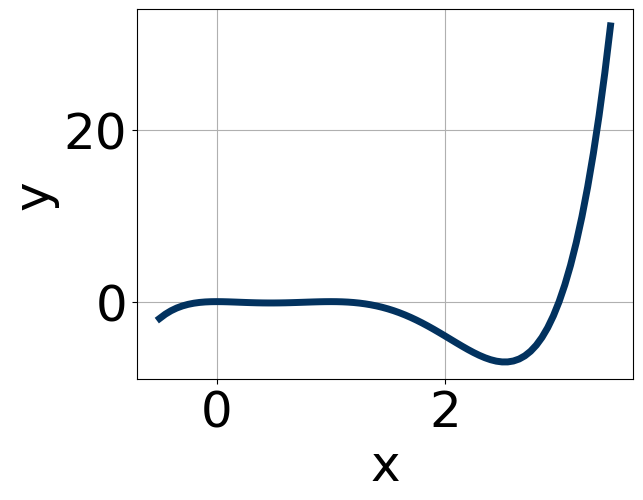
\includegraphics[width=0.5\textwidth]{../Figures/polyGraphToFunctionC.png}
\end{center}


The solution is \( 9x^{4} (x - 1)^{10} (x - 3)^{9} \), which is option C.\begin{enumerate}[label=\Alph*.]
\item \( 6x^{9} (x - 1)^{4} (x - 3)^{5} \)

The factor $x$ should have an even power.
\item \( 19x^{11} (x - 1)^{8} (x - 3)^{6} \)

The factor $x$ should have an even power and the factor $(x - 3)$ should have an odd power.
\item \( 9x^{4} (x - 1)^{10} (x - 3)^{9} \)

* This is the correct option.
\item \( -8x^{10} (x - 1)^{8} (x - 3)^{7} \)

This corresponds to the leading coefficient being the opposite value than it should be.
\item \( -11x^{4} (x - 1)^{8} (x - 3)^{8} \)

The factor $(x - 3)$ should have an odd power and the leading coefficient should be the opposite sign.
\end{enumerate}

\textbf{General Comment:} General Comments: Draw the x-axis to determine which zeros are touching (and so have even multiplicity) or cross (and have odd multiplicity).
}
\end{enumerate}

\end{document}